\section{Timing Cuts}

There are several approaches used historically to identify hadrons in CLAS, all of them rely on time-of-flight information.  Before applying timing cuts, timing information is corrected following the method of Nathan Harrison (cite here).  This method involves (details here).   \\

% ----------------------------------------------------
%     tof-mass cut 
% ----------------------------------------------------
\subsection{Time of Flight Mass Cut}

The mass of a particle can be calculated using the time of flight information and the start time of the event,

\begin{equation}
  M_{ToF} = p \; \frac{1 - \beta^2}{\beta^2}
\end{equation}

Where $\beta = \frac{d}{(t_{hit}-t_{start}) c}$ and $t_{start} = t_{e} - d/v_{e}$.  All timing information used in these calculations is corrected as described above.  Linear boundaries can be used to cut around the mass of a particle of interest, in our case the kaon mass.  As with other timing cuts, separation of pions and kaons becomes difficult at higher momentum.  Time of flight mass cuts have the advantage that for weak signals the boundaries are easy to draw, where fitting the $\beta (p)$ distribution might be difficult.  This cut has a disadvantage as compared with the $\beta (p)$ cut (below) that $M_{ToF}$ not only contains detector information from time of flight but also from drift chambers in the momentum term.  In this analysis, a time of flight mass cut is considered.  The upper boundary $M_{ToF} < 0.75 \; GeV/c^{2}$ is not difficult to place, because for the negative case there is not a heavier background, and for the positive case protons lie far enough away.  The lower boundary is the critical boundary in order to maximally separate kaons from the lighter pions.  \\

In order to choose the lower boundary, the time of flight mass is sliced into different momentum bins.  Each slice is then fit with a double Gaussian over the neighboring pion-kaon mass peaks.  If the fit quality is good, the individual Gaussian fits are interpreted as the mass distribution of each particle in the sample.  Using this information, the kaon efficiency is defined.

\begin{equation}
  \mathcal{\epsilon}_{K^{\pm}} = \frac{\int_{M_{cut}}^{M_{upper}} f_{K^\pm}(M) dM }{\int_{M = 0.0}^{M_{upper}} f_{K^\pm}(M) dM }
\end{equation}

Where $f_{K\pm}$ is the fit to the kaon mass peak for positive/negative charge.  The efficiency represents the fraction of kaons that we identify with a given value of $M_{cut}$. The pion contamination is defined as,

\begin{equation}
  C_{\pi^{\pm}} = \frac{\int_{M_{cut}}^{M_{upper}} f_{\pi^\pm}(M) dM }{\int_{M_{cut}}^{M_{upper}} f_{K^\pm}(M) +  f_{\pi^\pm}(M) dM }
\end{equation}

and represents the fraction of the total sample that is pion background.


\begin{figure}
  \begin{centering}
    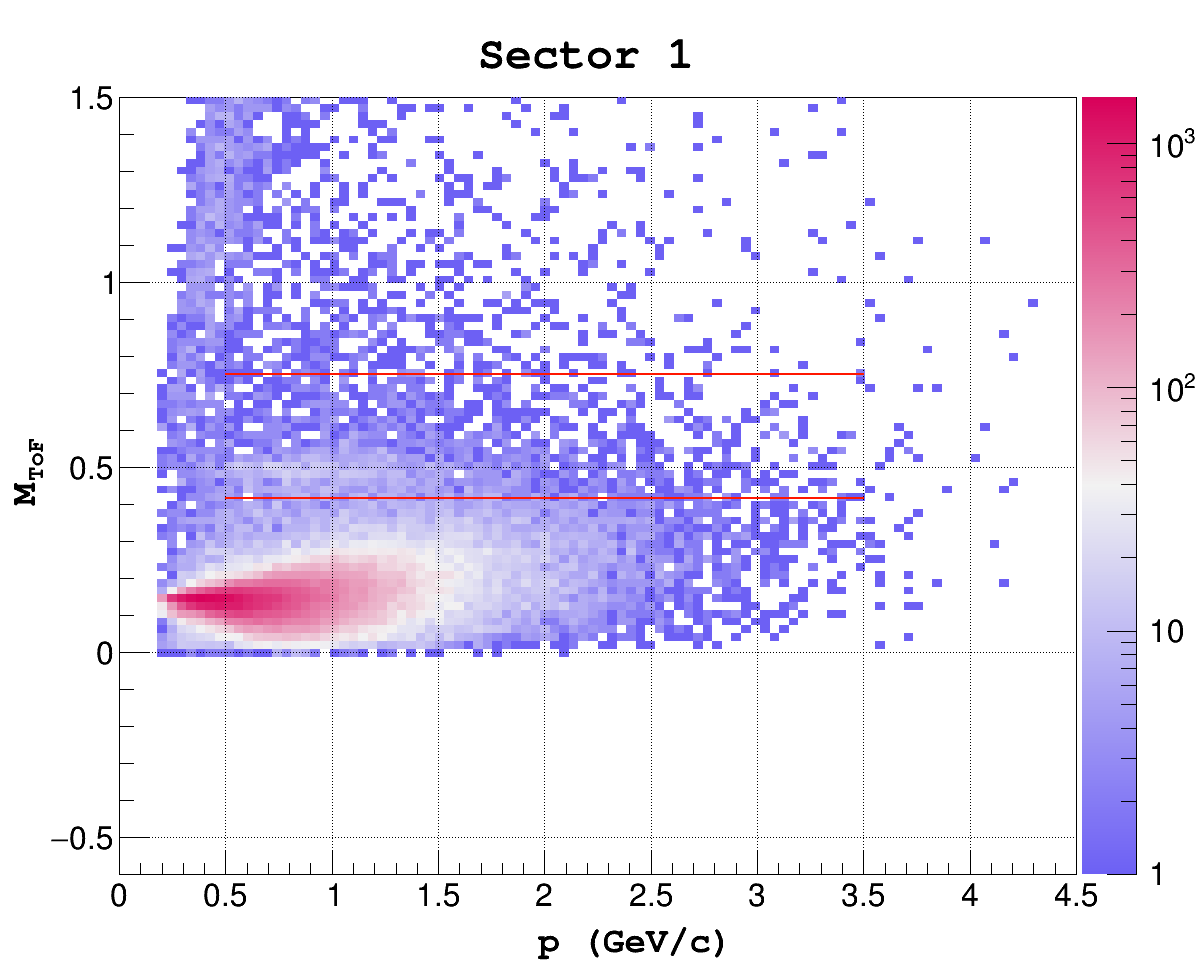
\includegraphics[width=10cm]{image/km/TofMassSector1.png}
    \caption{Time of flight mass shown for positive tracks in sector 1.}
  \end{centering}
\end{figure}


% ----------------------------------------------------
%          beta vs. p cut 
% ----------------------------------------------------
\subsection{$\beta$ Cut (Momentum Dependent)}

The calculation of the quantity $\beta$ was described above, using only time of flight information for the electron and hadron candidate.  Particles of mass $m$ show up in lines of constant mass from the equation below.  This can also be observed from figure \ref{fig:kp_bvp}. 

\begin{equation}
  \frac{p}{E} = \beta = \frac{p}{\sqrt{p^{2} + m^{2}}} 
\end{equation}

While the signal particle is more difficult to extract from these lines, the distribution is not skewed by information from the drift chambers momentum.    





